\begin{frame}{OpenVDB}
\begin{columns}
\column{0.58\linewidth}
\centering
\begin{outline}
    \1 Published in ACM Trans. Graphics 2013 \cite{Museth2013}
    \1 Work was completed at Dreamworks animation
    \1 Widely used for special effects and animation
      \2 Supported by industry standard software like Houdini and Blender
    \1 Describes VDB Datastructure
    \1 Introduced OpenVDB implementation
    \1 Often used with implicit geometry
\end{outline}
\column{0.38\linewidth}
\centering
\shadowimage[width=2.5cm]{vdb_paper.png}

\includegraphics[width=4cm]{open_vdb_puss_in_boots.png} 

\end{columns}

\end{frame}

\begin{frame}{VDB Datastructure}
\begin{columns}
\column{0.48\linewidth}
\centering
\begin{outline}
    \1 Similar to B+Trees
    \1 Dynamic root branching factor
      \2 Hashing
      \2 Virtually infinite
    \1 Fixed height, large branching factors
    \1 Constant time 
    \1 Large, dynamic branching factor 
\end{outline}
\column{0.48\linewidth}
\centering
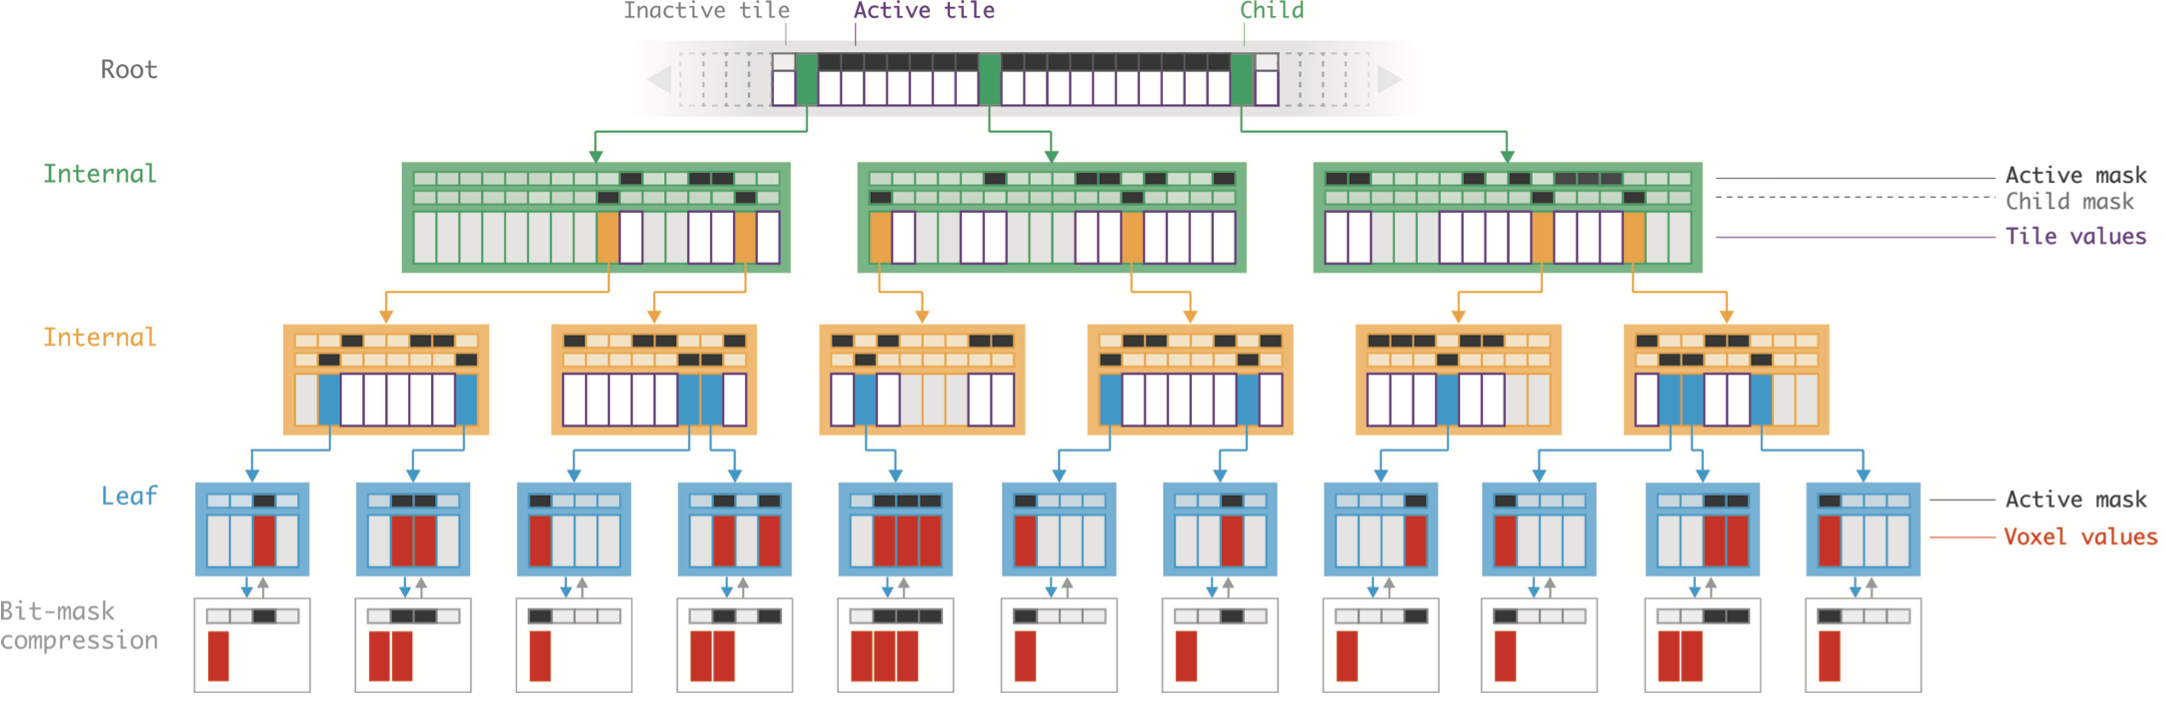
\includegraphics[width=5cm]{open_vdb_data_structure.png}

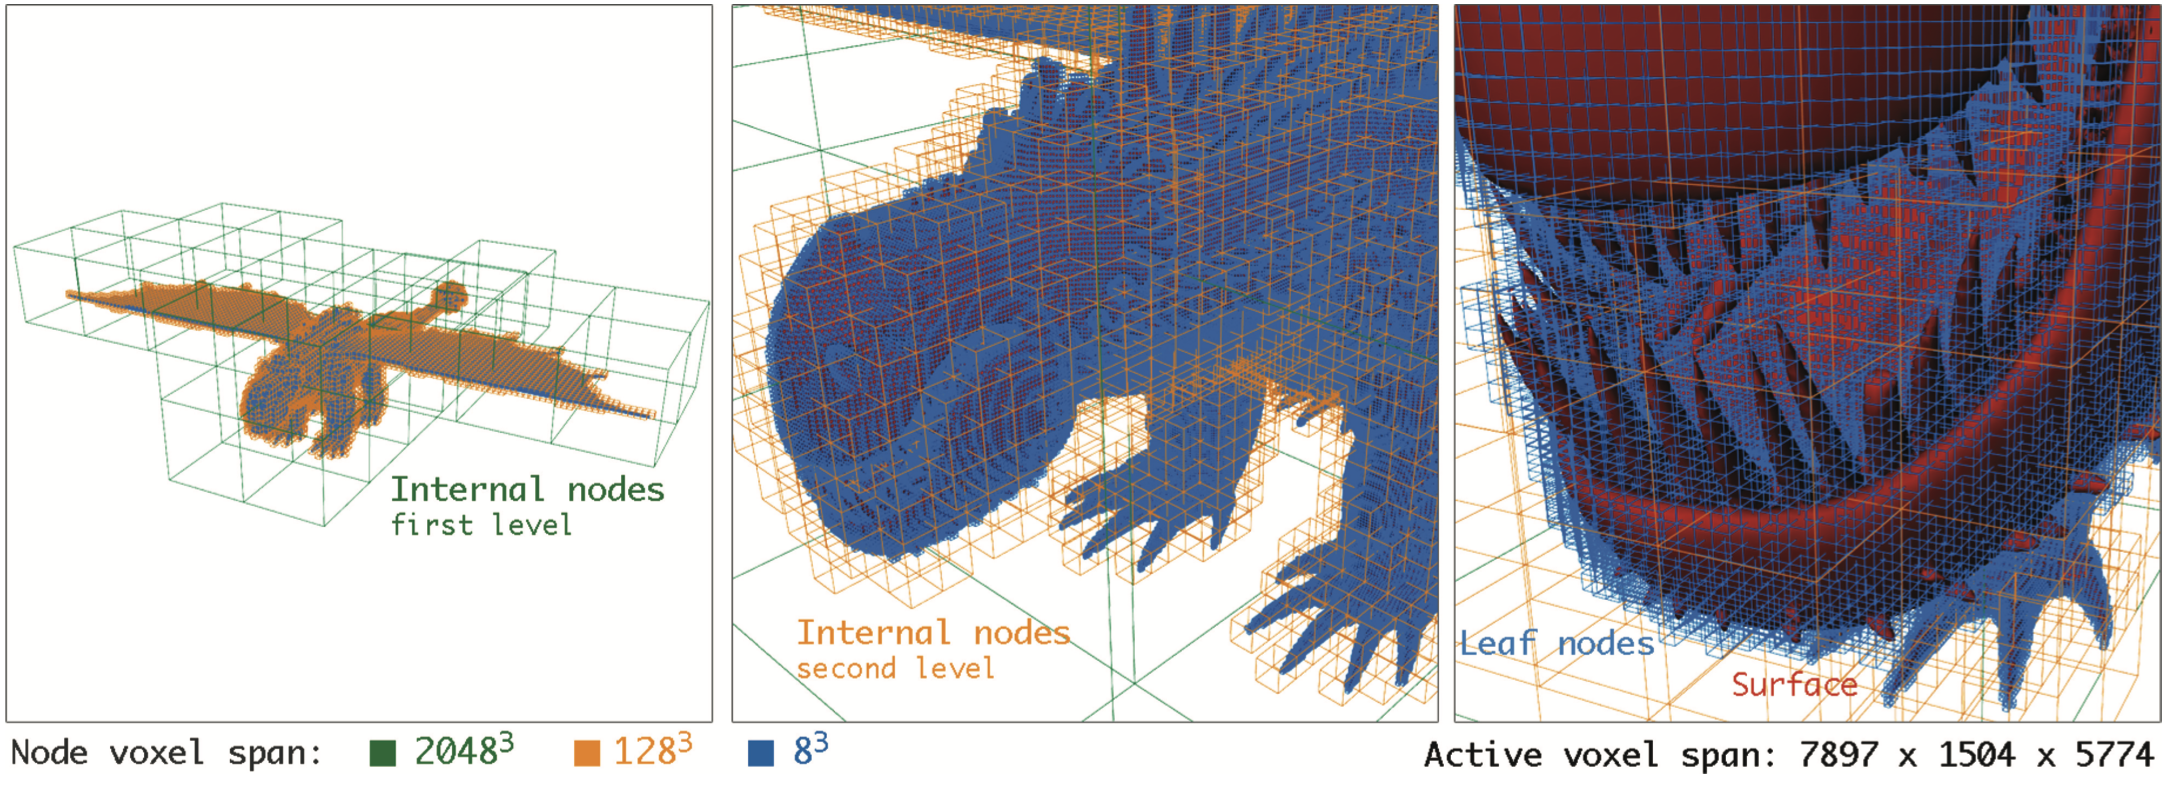
\includegraphics[width=5cm]{open_vdb_visual_aid.png} 


\end{columns}

\blfootnote{Images from \cite{Museth2013}}
\end{frame}
